\section{商业模式展望}

下面将简要地讨论五个课题:
\begin{itemize}
    \item 第一个课题考察超越经济利益的商业模式:商业模式画布如何在公共服务和非营利组织中推动商业模式创新。
    \item 第二个课题探讨计算机辅助的商业模式设计相对于笔头设计的优势,允许我们更复杂地操纵商业模式元素。
    \item 第三个课题讨论商业模式和商业计划之间的关系。
    \item 第四个课题则指出在初创组织或者成熟组织中执行商业模式的时候会出现的问题。
    \item 第五个课题考察如何更好地协同商业模式和IT。
\end{itemize}

\subsection{超越经济利益的商业模式}
\begin{itemize}
    \item 每一个组织都有一个商业模式,即便它并没有“商业”属性
    \item 为非盈利组织、慈善机构、公共服务实体和以盈利为目的的社会投资机构服务
    \item 主要讨论的是非盈利组织的的商业模式,这种我们更倾向于叫做“企业模式”
    \begin{itemize}
        \item 第三方资助的企业模式(比如公益组织、慈善组织、政府组织)
        \item 有强烈的环境和社会使命的“三重损益商业模式:“三重损益”指的是计算环境、社会和财务成本
    \end{itemize}
\end{itemize}


\subsection{计算机辅助的商业模式设计}
\begin{figure}[H]
	\centering
	\vspace{-0.5em}
	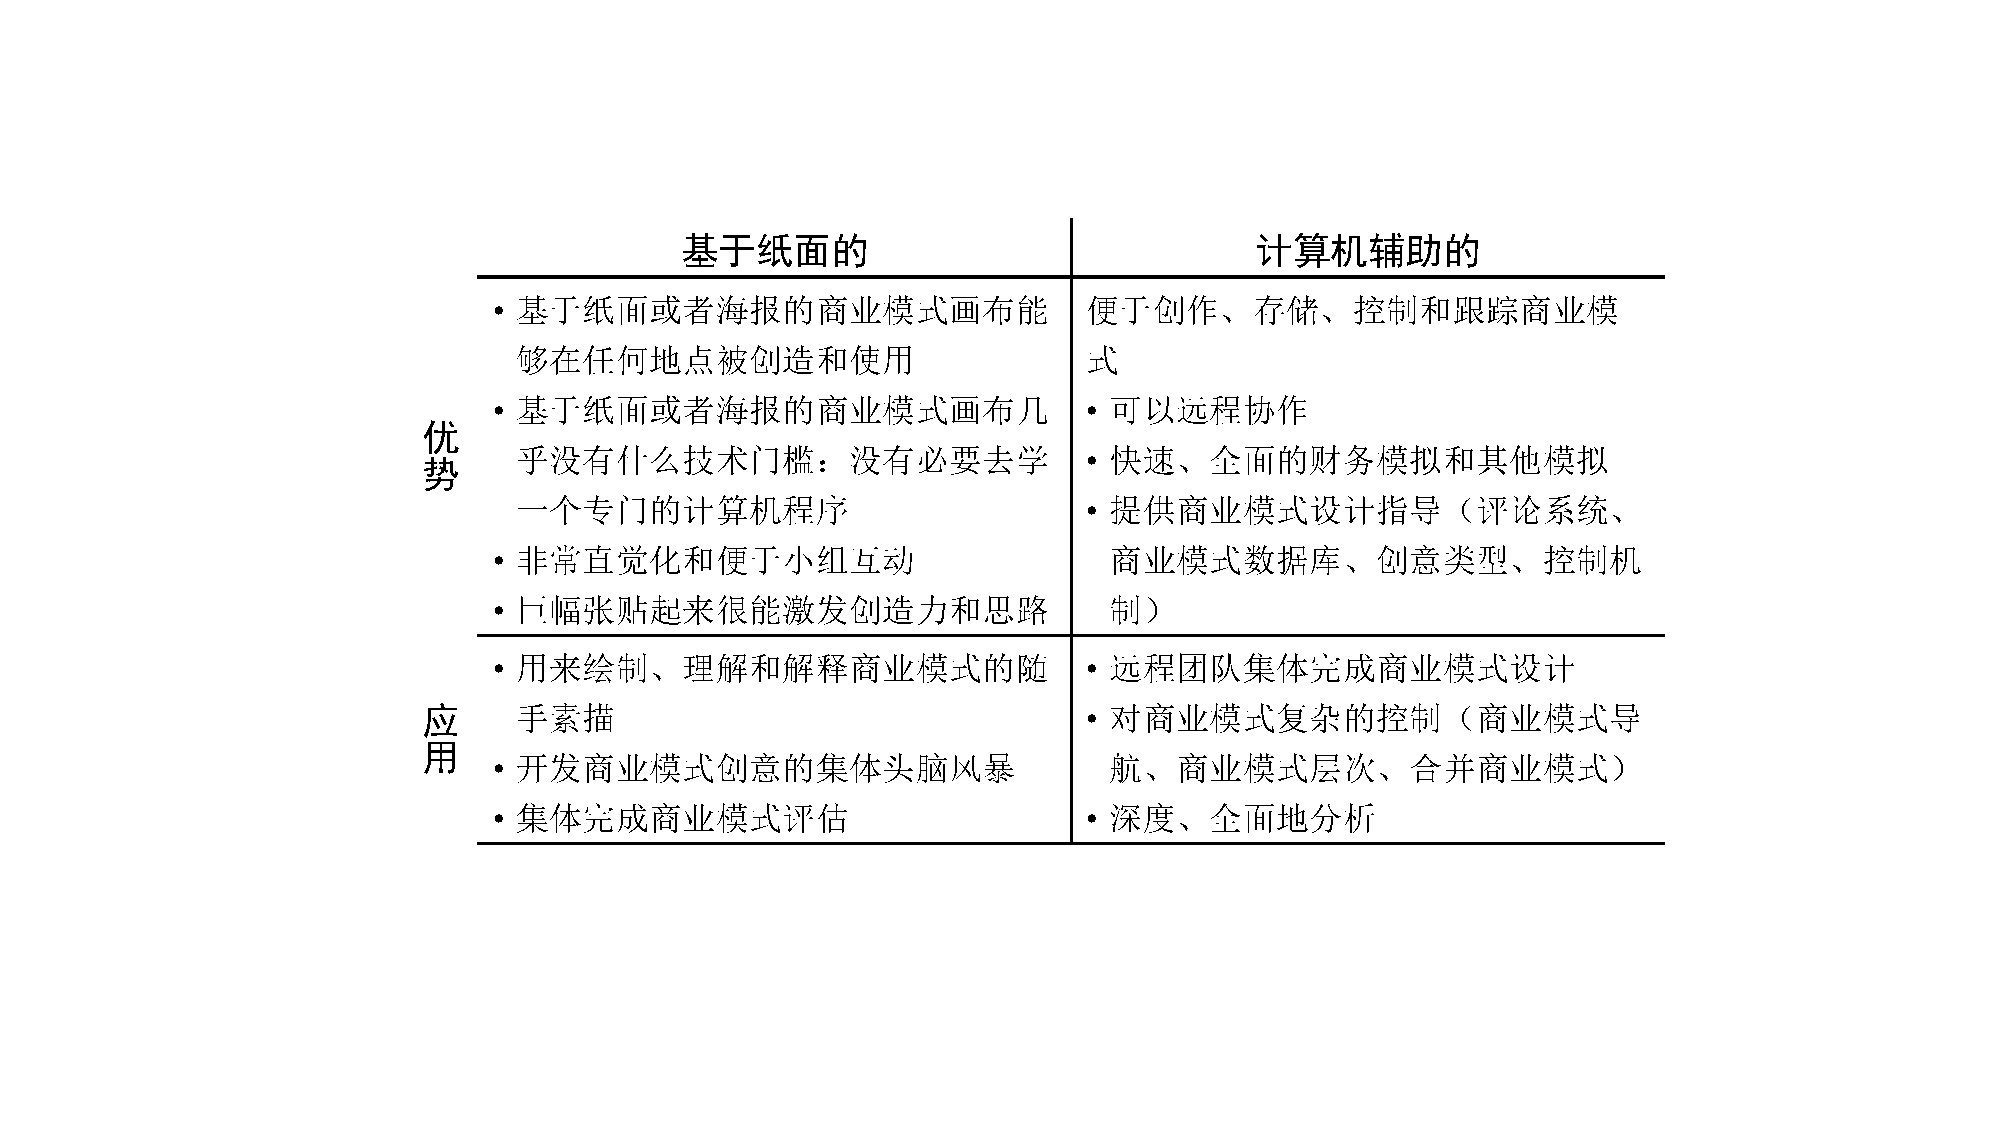
\includegraphics[width=0.65\textwidth]{img/计算机辅助的商业模式设计.pdf}
	\vspace{-0.5em}
\end{figure}

\subsection{商业模式和商业计划}
\begin{figure}[H]
	\centering
	\vspace{-0.5em}
	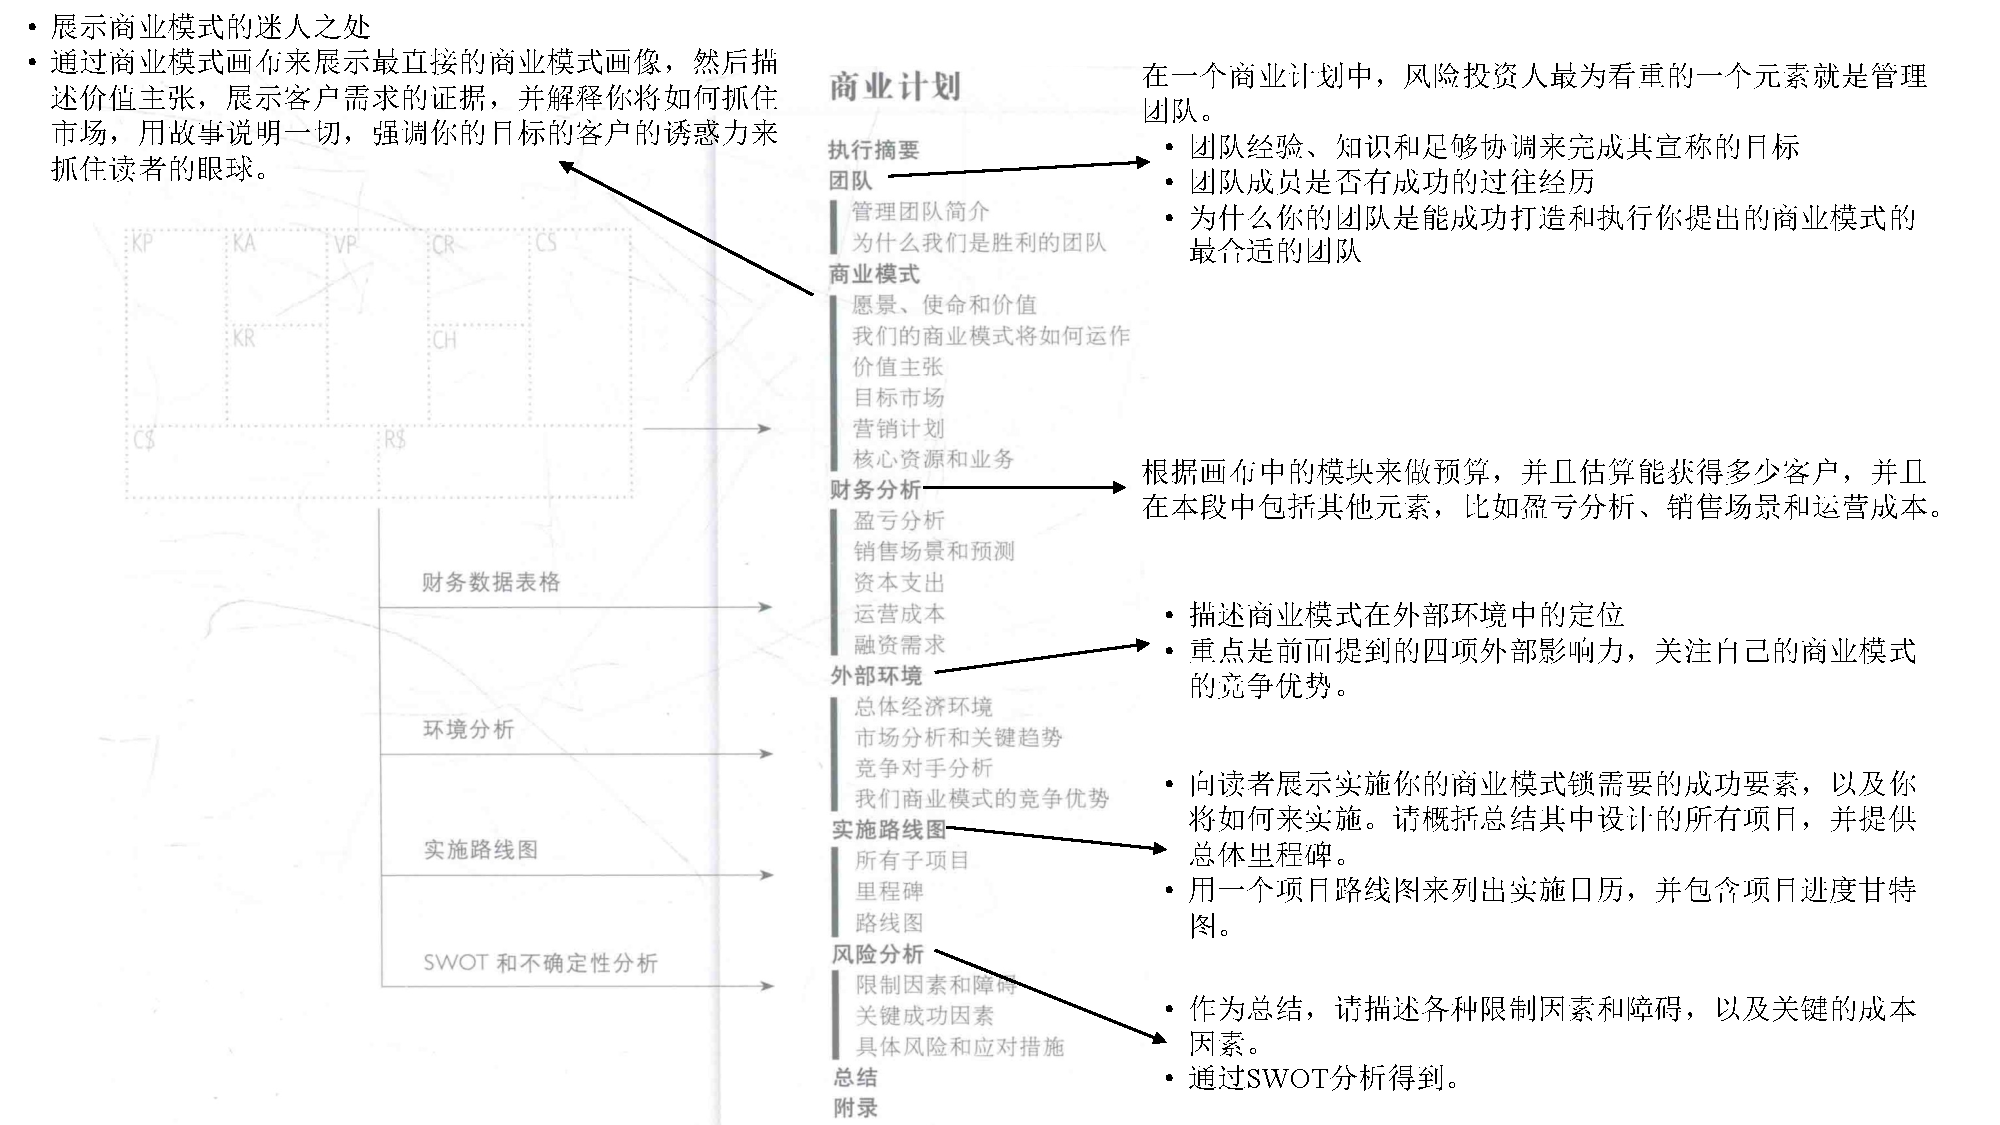
\includegraphics[width=\textwidth]{img/商业模式和商业计划.pdf}
	\vspace{-0.5em}
\end{figure}

\subsection{在组织中执行商业模式}
组织中必须相互协同的五个领域:战略、架构、流程、激励和人员。我们将商业模式放在这个星型的中央,好像一个“引力中心”牢牢抓住这五个领域。
\begin{figure}[H]
	\centering
	\vspace{-0.5em}
	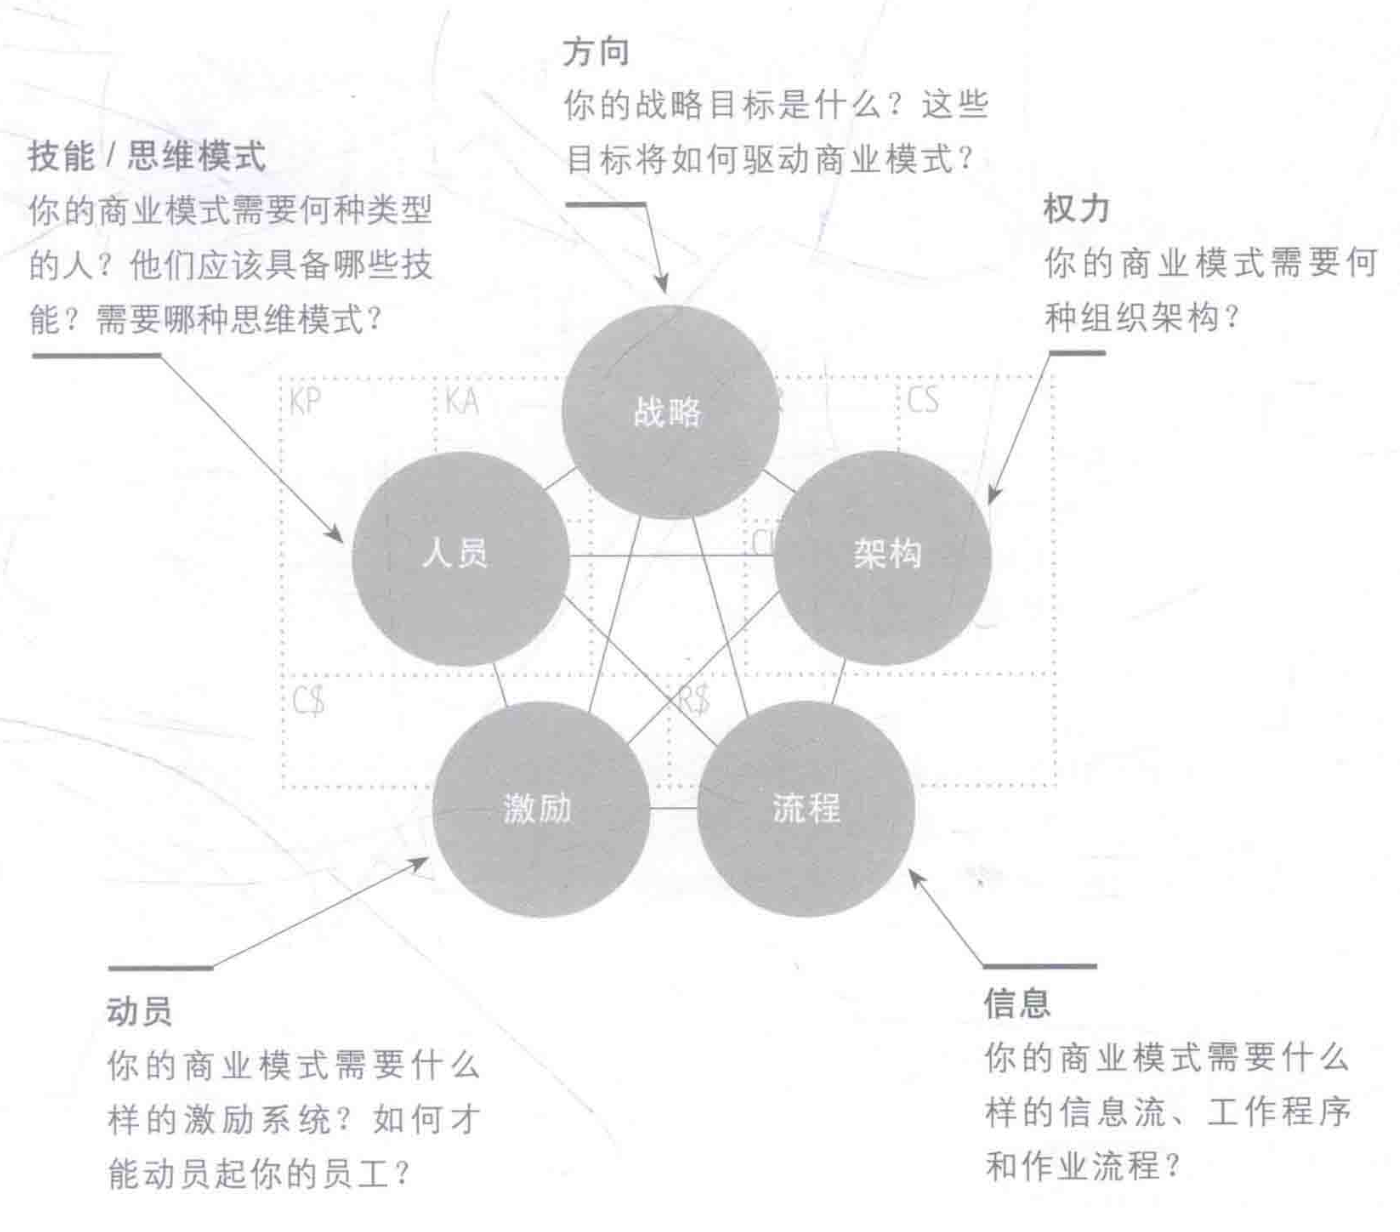
\includegraphics[width=0.6\textwidth]{img/在组织中执行商业模式.png}
	\vspace{-0.5em}
\end{figure}


\subsection{IT与业务的协同}
\begin{figure}[H]
	\centering
	\vspace{-0.5em}
	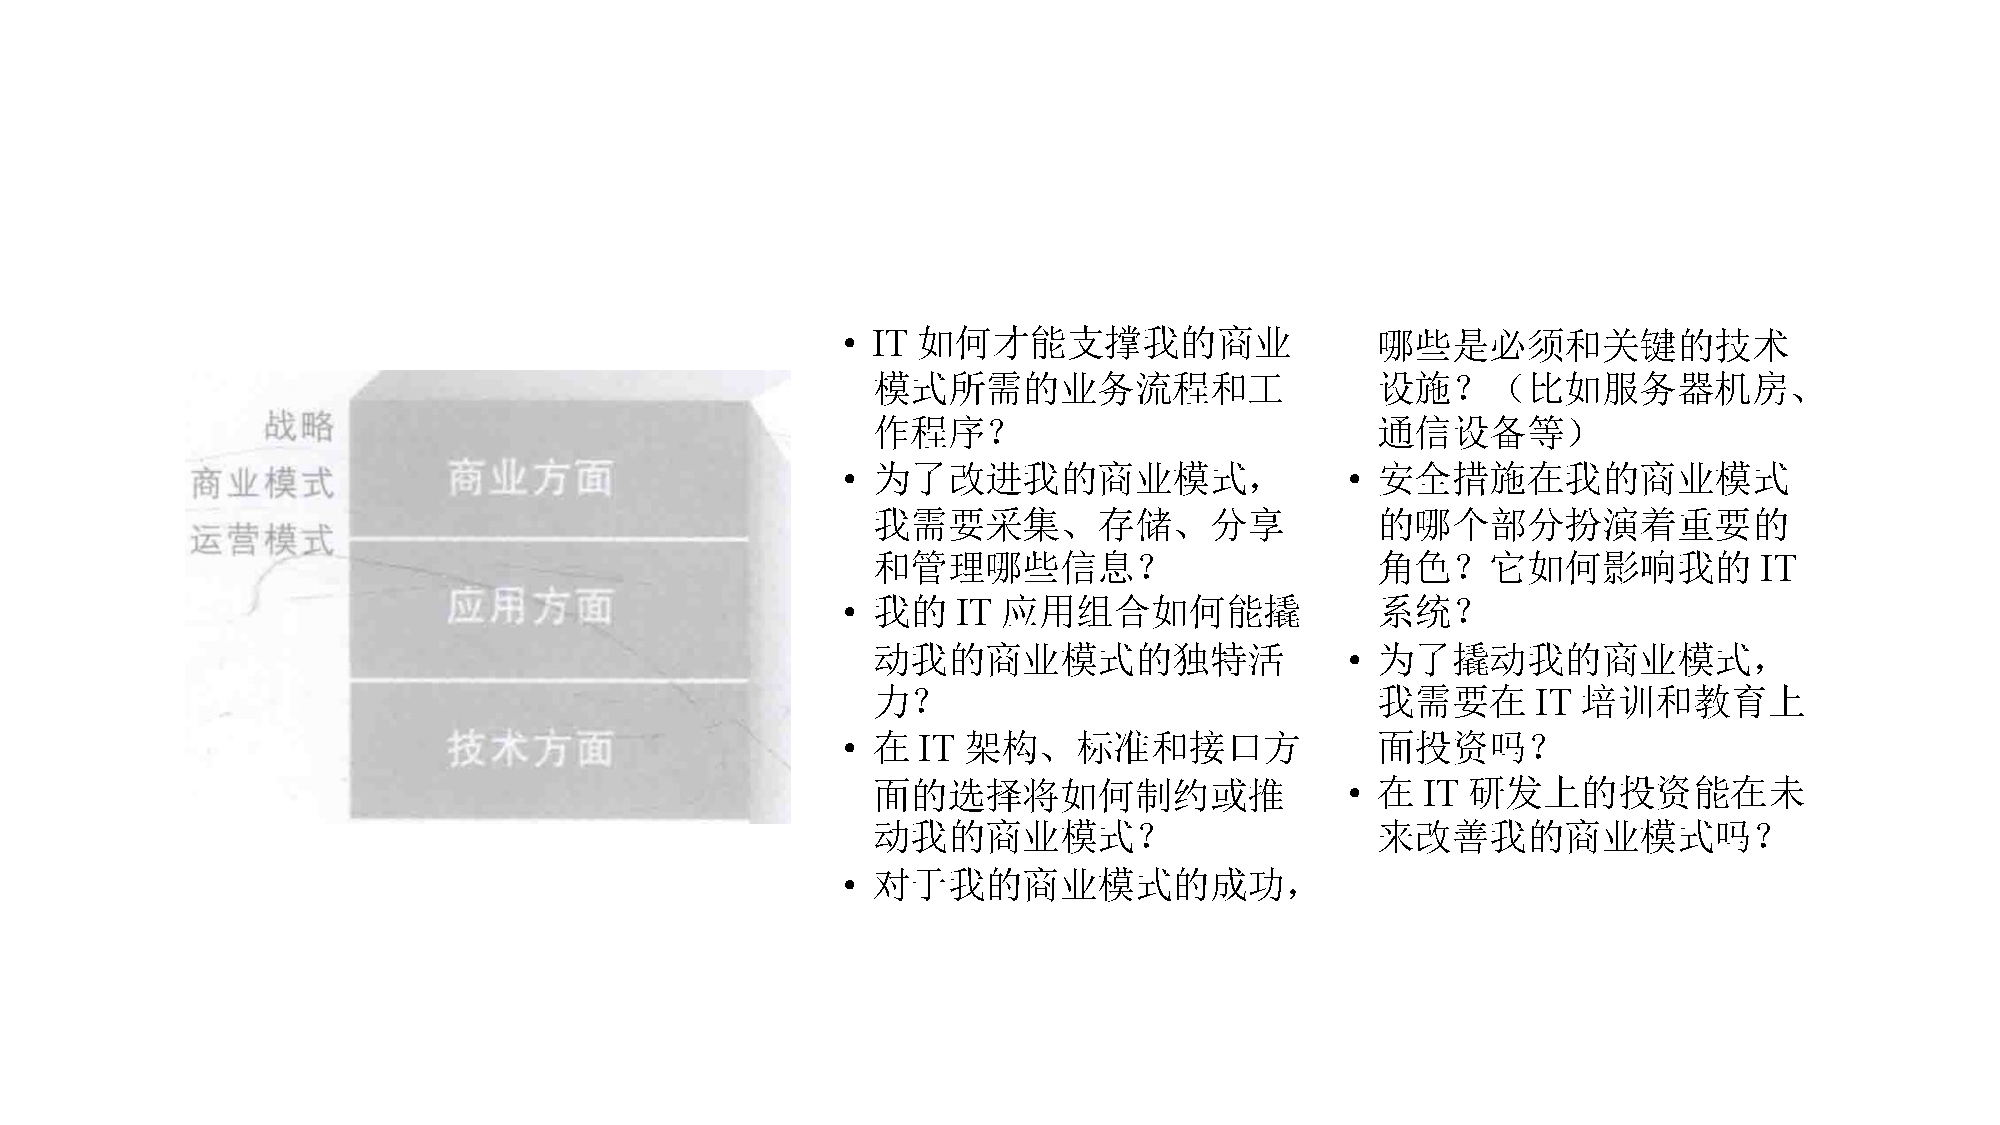
\includegraphics[width=0.85\textwidth]{img/IT与业务的协同.pdf}
	\vspace{-0.5em}
\end{figure}
	